\documentclass{beamer}

\usepackage{graphicx}
\usepackage{tabularx}
\usepackage[british]{datetime2}
\usetheme{default}
\usecolortheme{seagull}
\usepackage{newtxtext}
\setbeamertemplate{navigation symbols}{} % No navigation symbols
\usetheme{default}
\setbeamertemplate{navigation symbols}{} % No navigation symbols
% Comment this line for default bullet points (triangles)
\setbeamertemplate{itemize item}{\color{white}$\bullet$} 

\setbeamertemplate{footline}{
\begin{tabularx}{\textwidth} {
	 >{\raggedright\arraybackslash}X 
  	 >{\centering\arraybackslash}X 
  	 >{\centering\arraybackslash}X 
  	 >{\centering\arraybackslash}X
  	 >{\centering\arraybackslash}X 
  	 >{\centering\arraybackslash}X}
	
	\insertshortauthor & 
	\insertshorttitle &
	\insertdate &
	\insertsection &
	\insertframenumber /\inserttotalframenumber
\end{tabularx}
}

\makeatletter
\makeatother

\title[ISA 2023]{Historical Statehood and Organized Violence}

\subtitle{ISA 2023}

\author[Wishman]{Marius Swane Wishman} 
\date{\today} 
\institute{NTNU}

\begin{document}

\begin{frame}[plain]
\titlepage 
\end{frame}

\section{The Puzzle}

\begin{frame}
	\centering
	\Large The Puzzle
\end{frame}

\begin{frame} 
	\centering
	\Large ``What determines when and where pre-colonial
	statehood is conflict inducing or peace inducing?"

\end{frame}

\section{The Answer}

\begin{frame} 
	\centering
	\Large It depends...
\end{frame}

\begin{frame}{It depends...}
	\centering
	\Large ...On the relationship between the pre-colonial state and the
	post independence state
\end{frame}

\begin{frame}
	\begin{figure}
		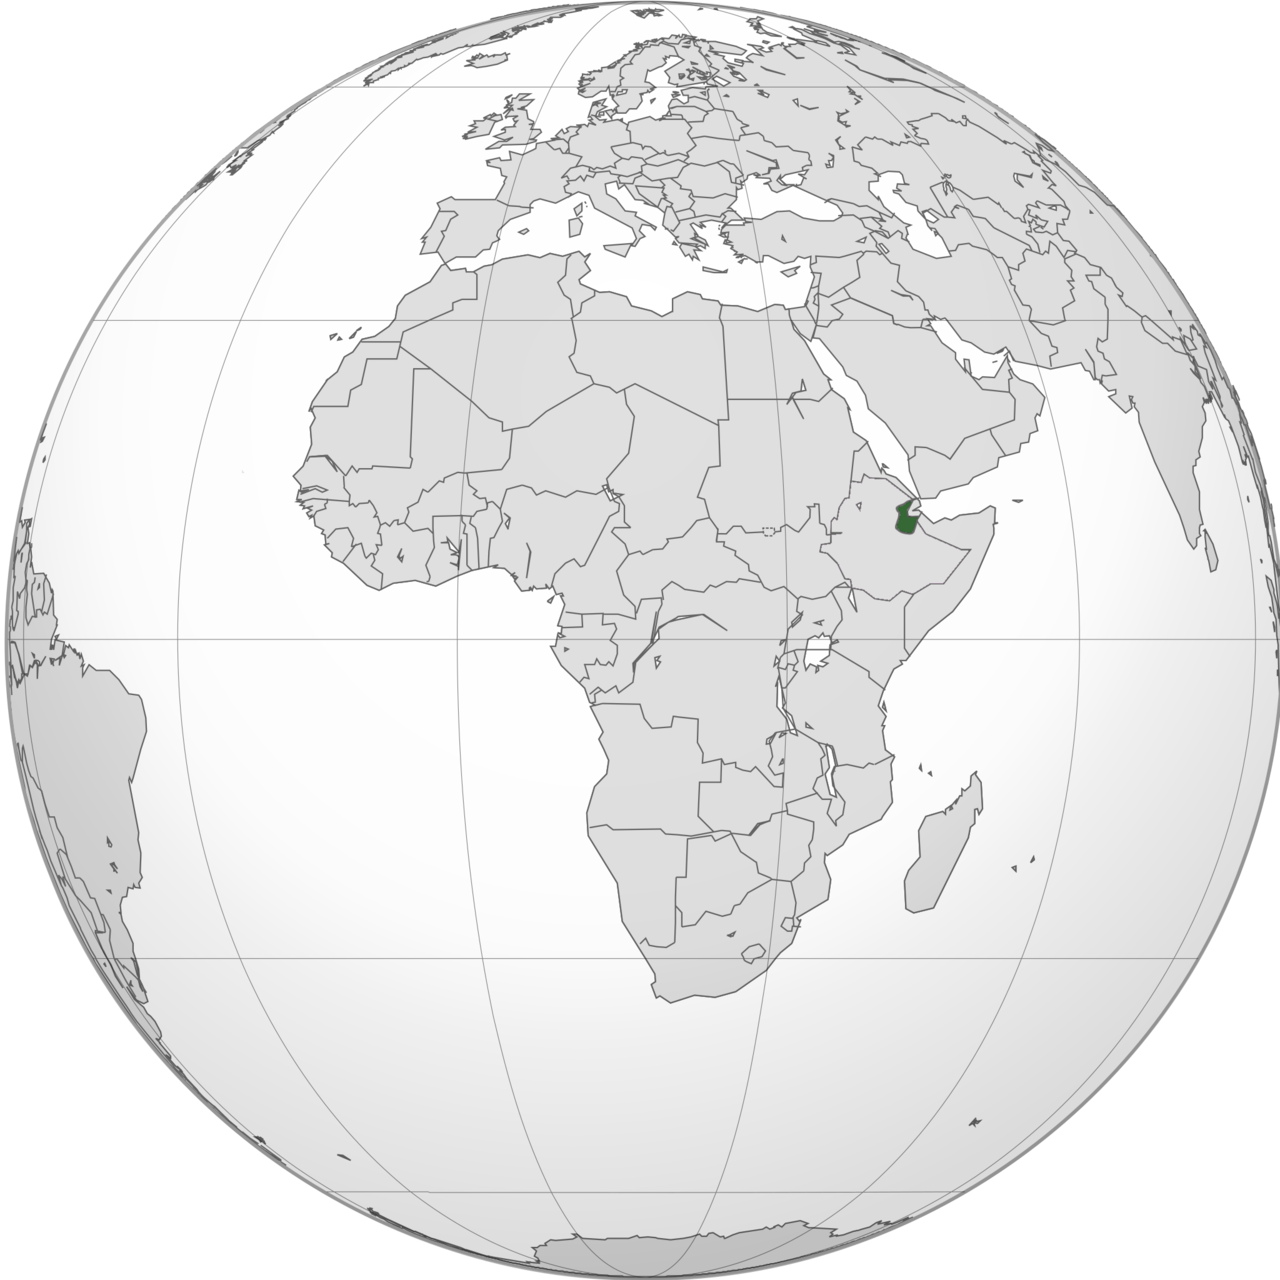
\includegraphics[width=.7\linewidth]{img/aussa.png}
	\end{figure}
\end{frame}

\begin{frame} Ouagadougou
	\begin{figure}
		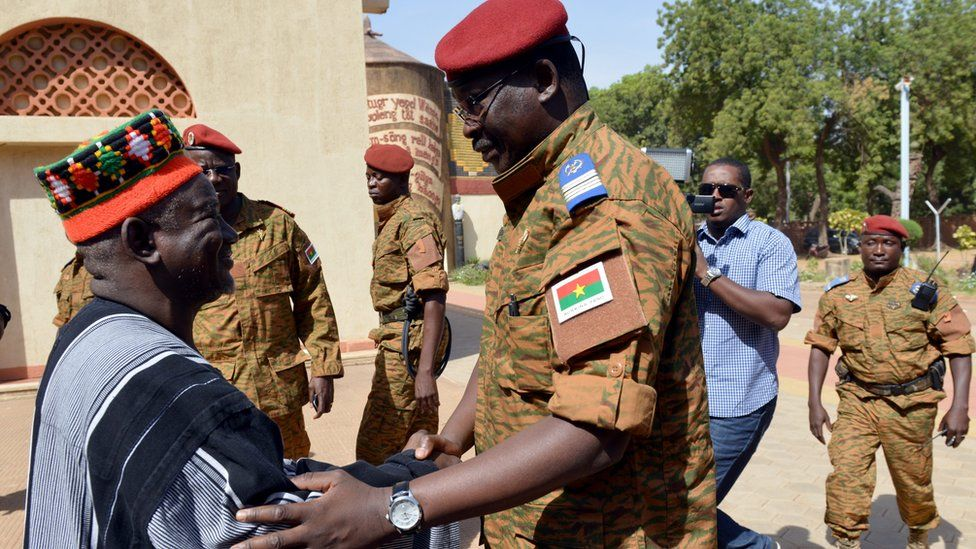
\includegraphics[width=\linewidth]{img/moghonaba.jpg}
	\end{figure}
\end{frame}

\begin{frame} % African sample
	\begin{figure}
		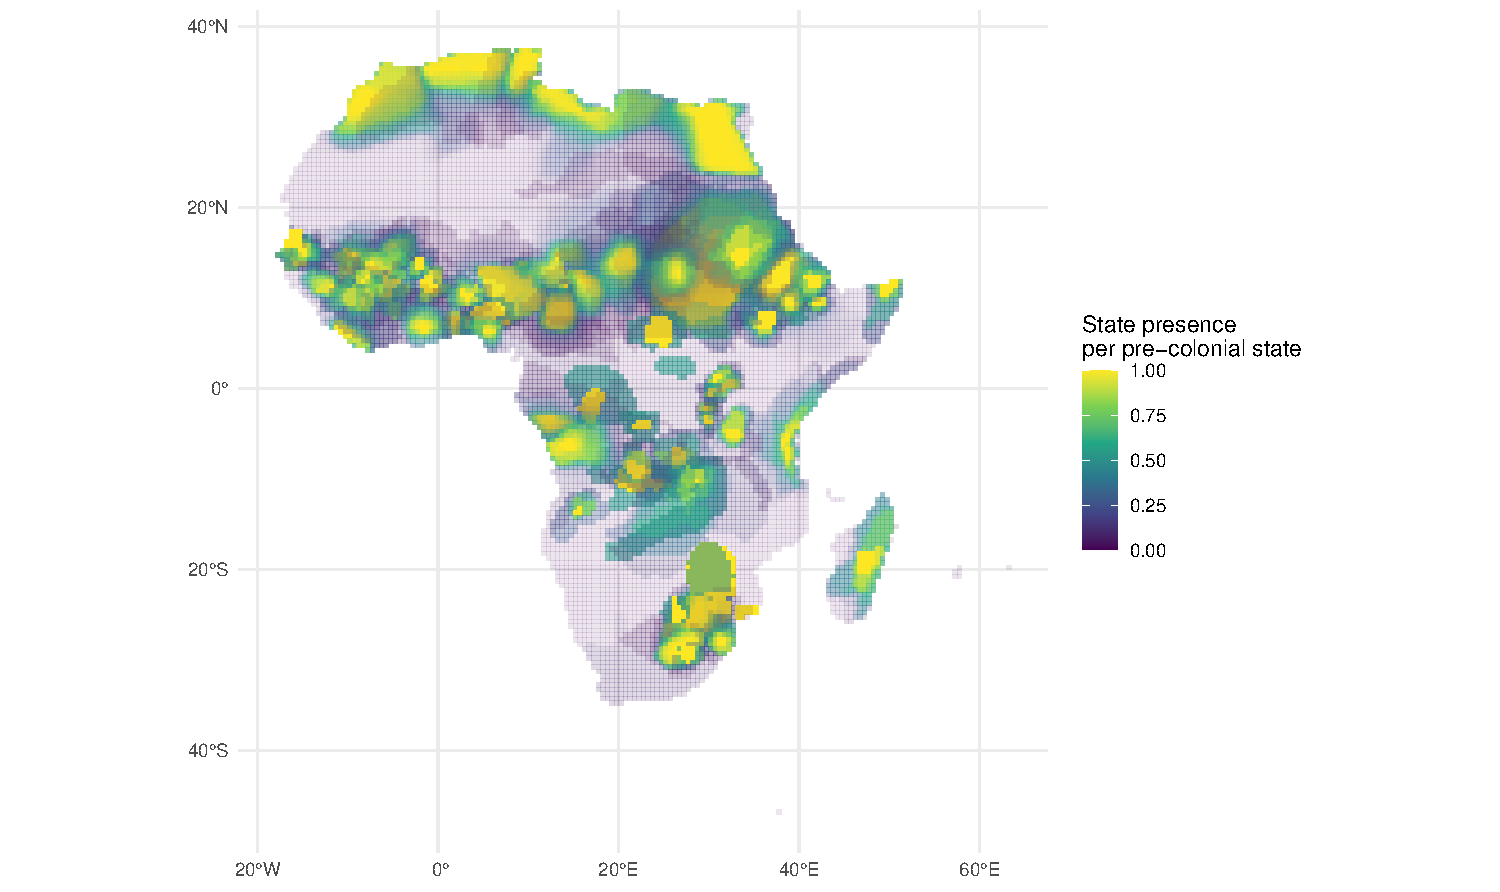
\includegraphics[width=\linewidth]{img/geo_isd_all.pdf}
	\end{figure}
\end{frame}

\begin{frame} % Nigeria
	\begin{figure}
		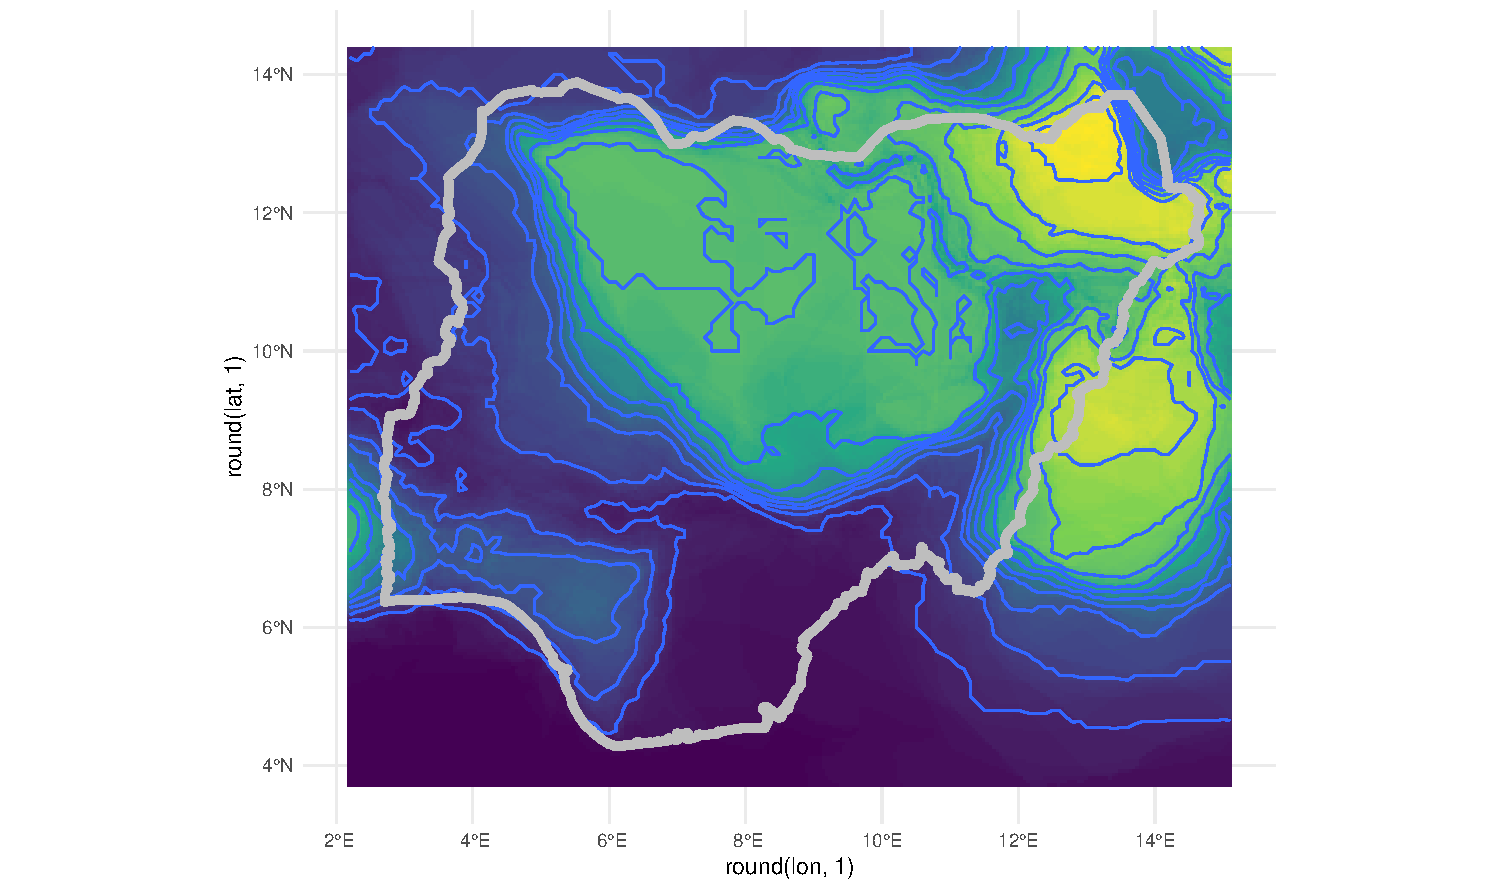
\includegraphics[width=\linewidth]{../R/Output/nigeria.pdf}
	\end{figure}
\end{frame}

\section{Results}

\begin{frame}
	\begin{figure}
		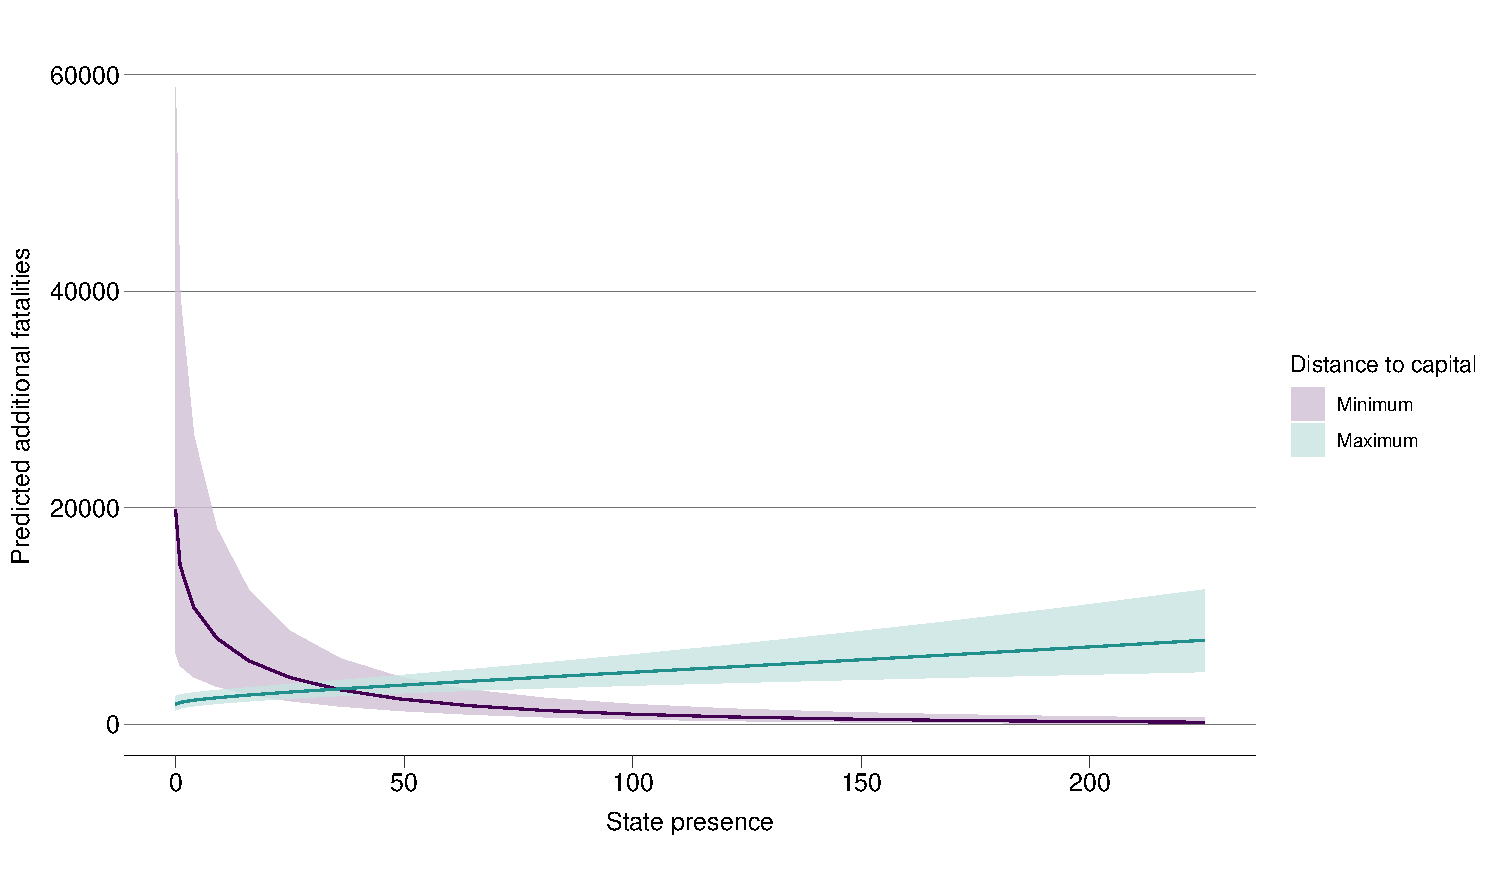
\includegraphics[width=\linewidth]{"../R/Output/interdeathszinbplot.pdf"}
	\end{figure}
\end{frame}

\section{Remaining work}

\begin{frame}{Remaining work}
	\begin{itemize}
		\item[-] Sensitivity test \pause
		\item[-] Control for overlap between current and historical
			capitals \pause
		\item[-] Different (larger) grid cells and regions \pasue
		\item[-] Better control for historical conflict (if I can find
			better data) \pause
		\item[-] Include more African scholars
	\end{itemize}
\end{frame}

\end{document}
